\section{Unterteilung der Streamingverfahren}
\subsection{Unterteilung nach Anwendnug}
\slides{it2-15-streaming_print}{3}
\subsection{Unterteilung nach Techniken}
\slides{it2-15-streaming_print}{4}
\subsection{Streaming mittels Webserver}
\slides{it2-15-streaming_print}{5}
\subsection{Dedizierte Streaming Protokolle}
\slides{it2-15-streaming_print}{6}
\section{Progressiver Download}
\slides{it2-15-streaming_print}{7}
\section{HTML mit Video-Tag}
\slides{it2-15-streaming_print}{8}
%%%% Einschub ch3
\section{HTTP-Pseudo-Streaming}
\lecdate{07.11.2017-1}
\slides{it2-15-streaming_print}{9}
\slides{it2-15-streaming_print}{10}
\slides{it2-15-streaming_print}{11}
\subsubsection*{Beispiel}
\slides{it2-15-streaming_print}{12}

\section{Dynamic Adaptive Streaming over HTTP (MPEG-DASH)}
\slides{it2-15-streaming_print}{13}
\subsection{Schema}
\slides{it2-15-streaming_print}{14}
\slides{it2-15-streaming_print}{15}
\subsection{MPD}
\slides{it2-15-streaming_print}{16}

\section{Streaming mit dediziertem Server}
\slides{it2-15-streaming_print}{19}
\subsection*{Client-Puffer}
\slides{it2-15-streaming_print}{20}

\section{Vergleich UDP und TCP}
\slides{it2-15-streaming_print}{21}

\section{Sonstiges}
\subsection{Schwankende Datenraten}
\slides{it2-15-streaming_print}{22}

\subsection{Steuerung des Abspielens}
\slides{it2-15-streaming_print}{23}

\subsection{Vergleich der Streaming-Techniken}
\slides[1]{it2-15-streaming_print}{24}
\begin{center}
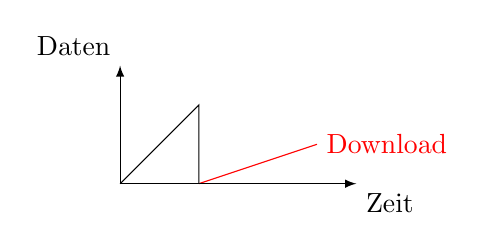
\begin{tikzpicture}[scale=1]
\draw (0,0) -- (1,1) -- (1,0);
\draw [red] (1,0) -- (2.5,0.5) node[right]{Download};
\draw [-latex] (0,0) -- (0,1.5) node[above left]{Daten};
\draw [-latex] (0,0) -- (3,0) node[below right]{Zeit};
\end{tikzpicture}
\end{center}
\begin{center}
\begin{tikzpicture}[scale=1]
\draw (0,0) -- (1,1) -- (1,0);
\draw [red] (0,0) -- (1.5,0.5) node[right]{progressiever Download};
\draw [-latex] (0,0) -- (0,1.5) node[above left]{Daten};
\draw [-latex] (0,0) -- (3,0) node[below right]{Zeit};
\fill [pattern= horizontal lines, pattern color = red] (0,0) -- (1,0.335) -- (0.33,0.335) -- cycle;
\end{tikzpicture}
\end{center}
\begin{center}
\begin{tikzpicture}[scale=1]
\draw (0,0) -- (1,1);
\draw [red] (0.5,0) -- (1.5,1) node[right]{Streaming};
\draw [-latex] (0,0) -- (0,1.5) node[above left]{Daten};
\draw [-latex] (0,0) -- (3,0) node[below right]{Zeit};
\fill [pattern= horizontal lines, pattern color = red] (0,0) -- (0.5,0) -- (1.5,1) -- (1,1) -- cycle;
\end{tikzpicture}
\end{center}

\section{Zusammenfassung}
\slides{it2-15-streaming_print}{25}










